\section{Totales Differential}
Wir wollen nun einen sinnvollen Begriff von Differenzierbarkeit für Funktinen oder Abbildungen die von mehreren Variablen abhängen definieren. Wir werden sehen, dass es nicht genügt, dass die partiellen Ableitungen existieren.

Was sich verallgemeinern lässt ist die Idee, eine Funktion durch eine affin-lineare Abbildung anzunähern, nämlich durch ihr erstes Taylorpolynom.

\begin{definition}{Totale Differenzierbarkeit}
	Eine Abbildung $f:E\rightarrow\R^m,E\subseteq \R^n$ heißt total differenzierbar in $x\in D$, falls eine Matrix $f'(x)=Df(x)\in M(m,n,\R)$ existiert, so dass
	\begin{equation*}
		f(x+h)=f(x)+f'(x)*h+o(h)
	\end{equation*}
	für alle $h\in\R^n, (x+h)\in D$ gilt. Hierbei muss die Restfunktion $o(h)\in\R^m$ die Bedingungen
	\begin{equation*}
		o(h)=r(x,h)*h\text{ mit }\lim\limits_{h\to 0} r(x,h)=0
	\end{equation*}
	erfüllen. Falls ein solches $f'(x)=Df(x)$ existiert, heißt es auch \emph{das totale Differential} von $f$ bei $x$.
\end{definition}

\paragraph{Beispiele:}
\begin{itemize}
	\item Es sei $\alpha=(\alpha_1,\ldots,\alpha_n)\in\R^n$ und sei $f:\R^n\rightarrow\R$ definiert durch
	\begin{equation*}
		f(x)=\alpha x+b = (\alpha_1,\ldots,\alpha_n)*\vector{x_1\\\vdots\\x_n}+b
	\end{equation*}
	Dies ist eine affin-lineare Abbildung. Dann ist $f'(x)=\alpha$ und zwar für alle $x\in\R^n$ gleichzeitig.
	Es gilt
	\begin{equation*}
		f(x+h)=\alpha (x+h)+b=\alpha x+\alpha h+b=f(x)+\alpha*h
	\end{equation*}
	das heißt wir lesen ab, dass $\alpha\in M(1,n,\R)$ das totale Differential $Df(x)$ für alle $x$ ist. Eine affin-lineare Abbildung hat konstante Ableitung.

	\item Funktioniert auch mit $f:\R^n\rightarrow\R^m, f(x)=Ax+b,A\in M(m,n,\R), b\in\R^m$ hierbei ist $Df(x)=A$ konstant.

	\item $f:\R^n\rightarrow\R, f(x)=x^T*x$ das heißt
	\begin{align*}
		f(x)&=(x_1,\ldots,x_n)\vector{x_1\\\vdots\\x_n}\\
		&=x_1^2+\ldots+x_n^2
		\intertext{wir erhalten}
		f(x+h)&=(x+h)^T*(x+h)\\
		&=x^Tx+x^Th+h^Tx+h^Th\\
		&=f(x)+2x^Th+h^Th
	\end{align*}
	also ist $2x^T\in M(1,n,\R)$ das totale Differential von $f$ bei $x$.
\end{itemize}

Um das totale Differential allgemein ausdrücken zu können, stellen wir nun einen Zusammenhang zur Richtungsableitung her.
\begin{satz}{}
	Sei $f:D\rightarrow\R$ mit $D\subseteq \R^n$ offen, bei $x\in D$ total differenzierbar, dann existiert die Richtungsableitung für beliebige $a\in\R^n$ bei $x$ und es gilt
	\begin{equation*}
		\frac{\partial f}{\partial a}(x)=Df(x)a
	\end{equation*}
\end{satz}
\begin{beweis}
	Wir setzen $h=t*h$ in die Definition ein und erhalten
	\begin{align*}
		f(x+h)&=f(x)+Df(x)*h+o(h)\\
		f(x+ta)&=f(x)+(Df(x)a)t+o(ta)
	\end{align*}
	\begin{equation*}
		\Rightarrow\enspace \frac{f(x+ta)-f(x)}{t}=Df(x)a+\frac{o(ta)}{t}
	\end{equation*}
	\ \hfill$\Box$
\end{beweis}

Wir haben gezeigt, dass die partielle Ableitung $\frac{\partial f}{\partial x_k}(x)$ ein Spezialfall der Richtungsableitung ist, nämlich für $a=e_k$ (kanonischer Basisvektor).
Dies zeigt, wie man das totale Differential berechnet, die Spalten von $Df(x)$ sind die partiellen Ableitungen von $f$.

Also gilt, falls $f:D\rightarrow\R, D\subseteq \R^n$ bei $x\in D$ total differenzierbar ist
\begin{equation*}
	\renewcommand{\arraystretch}{1.7}
	f'(x)=Df(x)=
	\begin{pmatrix}
		\frac{\partial f_1}{\partial x_1}(x) &\frac{\partial f_1}{\partial x_2}(x) &\cdots &\frac{\partial f_1}{\partial x_n}(x) &\\
		\frac{\partial f_2}{\partial x_1}(x) &\frac{\partial f_2}{\partial x_2}(x) &\cdots&\frac{\partial f_2}{\partial x_n}(x) &\\
		\vdots&\vdots&\ddots&\vdots\\
		\frac{\partial f_m}{\partial x_1}(x) &\frac{\partial f_m}{\partial x_2}(x) &\cdots&\frac{\partial f_m}{\partial x_n}(x) &
	\end{pmatrix}
\end{equation*}
Die Matrix $Df(x)$ heißt die \emph{Jacobimatrix} $\jacobi$ von $f$ bei $x$. Falls das Differential existiert, ist es durch die Jacobimatrix gegeben.

\paragraph{Beispiel:}
Sei $f:\R^2\rightarrow\R^2$ mit
\begin{equation*}
	f(x,y)=\matrix{x^2y\\x+\sin(y)}
\end{equation*}
dann ist die Jacobimatrix von $f$ bei $(x,y)$ gegeben durch
\begin{equation*}
	\jacobi f(x,y)=\matrix{2xy&x^2\\1&\cos(y)}
\end{equation*}

\paragraph{Bemerkungen:}
\begin{itemize}
	\item Wie bei Funktionen einer Variablen gilt: Aus (totaler) Differenzierbarkeit folgt Stetigkeit
	\item Ist $n>1$ also hat man mehrere Variable, dann folgt aus der Existenz aller partiellen Ableitungen bei $x\in D$ nicht die totale Differenzierbarkeit.

	Denn zum Beispiel ist die Funktion $f:\R^2\rightarrow \R$ mit
	\begin{equation*}
		f(x,y)=\begin{cases}
		0\text{, für } x=y=0\\
		\frac{x^5}{(y-x^2)^2+x^6}\text{, sonst}
		\end{cases}
	\end{equation*}
	nicht partiell differenzierbar in $x_0=(0,0)$, obwohl alle partiellen Ableitungen exisiteren.
	\begin{align*}
		\frac{\partial f}{\partial x}(0,0)
		&=\lim\limits_{h\to 0}\frac{f(h,0)-f(0,0)}{h} & \frac{\partial f}{\partial y}(0,0)&=\lim\limits_{h\to 0}\frac{f(0,h)-f(0,0)}{h}\\
		&=\lim\limits_{h\to 0}\frac{h^5}{h^5+h^7} & &=\lim\limits_{h\to 0}\frac{\frac{0}{h^2}}{h}\\
		&=\lim\limits_{h\to 0}\frac{1}{1+h^2} & &=\lim\limits_{h\to 0}\frac{0}{h^3}\\
		&=1 & &=0
	\end{align*}
	Auch außerhalb des Punktes $(0,0)$ exisiteren beide partiellen Ableitungen. Allerdings ist $f$ im Punkt $(0,0)$ nicht stetig, also insbesondere nicht total differenzierbar. Um dies zu zeigen sehen wir uns die Punkte $(h_1,h_2)=(h_1,h_1^2)$ an, die auf einem Parabelast liegen.
	Wir erhalten
	\begin{align*}
		&f(h,h^2)=\frac{h^5}{(h^2-h^2)^2+h^6}=\frac{h^5}{h^6}=\frac 1h
		\intertext{es gilt also für den Grenzwert}
		&\lim\limits_{h\to 0}\frac 1h \to\infty
	\end{align*}
	Das heißt, $f$ ist unstetig bei $x_0=(0,0)$!
\end{itemize}

\subsection{Gradient}
Für $m=1$, also reellwertige Funktionen ist $Df(x)=(\frac{\partial f}{\partial x_1}(x),\ldots,\frac{\partial f}{\partial x_n}(x))$ ein Zeilenvektor, das heißt eine $1\times n$-Matrix. Der Vektor
\begin{equation*}
	\nabla f(x)=\grad f(x)=\vector{\frac{\partial f}{\partial x_1}(x)\\\vdots\\\frac{\partial f}{\partial x_n}(x)}\in\R^n
\end{equation*}
wird in diesem Fall \emph{Gradient} von $f$ bei $x\in D\subseteq\R^n$ genannt.

Dieser Vektor zeigt in Richtung des steilsten Anstiegs der Funktion $f$.
\paragraph{Beispiel:}
$f:\R^2\rightarrow \R,(x,y)\mapsto x^2+y^2$ dann ist
\begin{equation*}
	\nabla f(x,y)=\vector{2x\\2y}
\end{equation*}
\begin{center}
	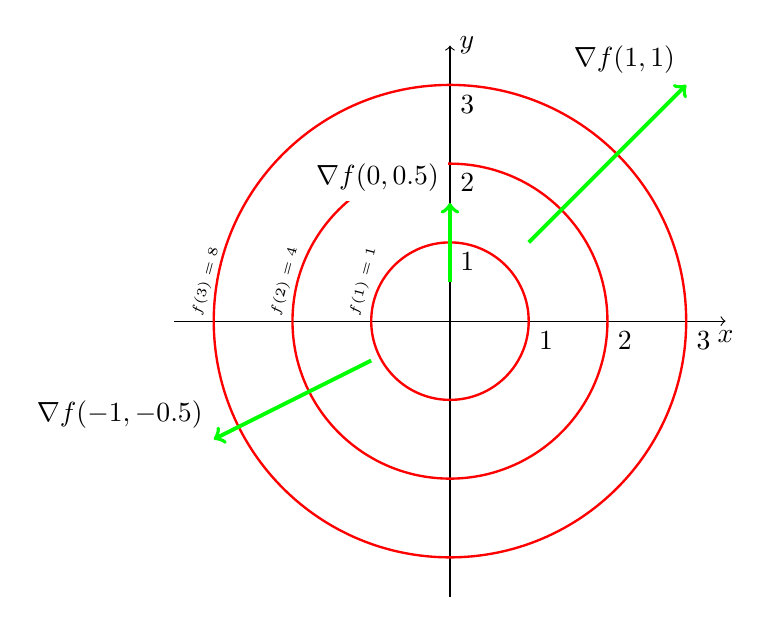
\begin{tikzpicture}

		\draw[->] (-3.5,0) -- (3.5,0) node[below] {$x$};
		\draw[->] (0,-3.5) -- (0,3.5) node[right] {$y$};

		\foreach \x in {1,2,3}
		\draw (\x,0) node[draw, inner sep=0pt, minimum size=0pt, minimum height = 4pt, label={below right:$\x$}] {};

		\foreach \x in {1,2,3}
		\draw (0,\x) node[draw, inner sep=0pt, minimum size=0pt, minimum width = 4pt, label={below right:$\x$}] {};

		\foreach \x in {1,2,3}
		\draw[red, line width=0.3mm] (0,0) circle (\x);
		\foreach \x/\y in {1/1,2/4,3/8}
		\draw (-\x-0.1,0.5) node[black, rotate=75] {\tiny$f(\x)=\y$};

		\foreach \x/\y in {1/1,0/0.5,-1/-0.5}
		\draw[green, ->, line width=0.5mm] (\x,\y) to (3*\x, 3*\y) node[above left, black, fill=white] {$\nabla f(\x,\y)$};
	\end{tikzpicture}
\end{center}

\subsection{Sätze zum totalen Differential}
\begin{satz}{}
	Existieren alle partiellen Ableitungen und sind diese stetig in $D$, dann ist die Ableitung $f:D\rightarrow\R^m$ total differenzierbar.
\end{satz}

\paragraph{Merkregel:}
\begin{center}
	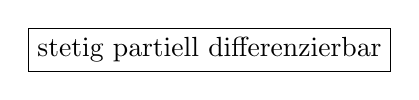
\begin{tikzpicture}
		\draw (0,0) node (spd) [draw] {stetig partiell differenzierbar};
	\end{tikzpicture}
\end{center}

\begin{satz}{Mittelwertsatz für reellwertige Funktionen}
	Sei $f:D\rightarrow\R,D\subseteq \R^n$ stetig differenzierbar in $D$ und $x,y$ sowie die Verbindungsstrecke $\overline{xy}=\set{x+t(y-x)}{t\in[0,1]}$ in $D$ enthalten. Dann exisitert ein $\xi\in\overline{xy}$, so dass
	\begin{equation*}
		f(y)-f(x)=Df(\xi)(y-x)
	\end{equation*}
	gilt. Dies verallgemeinert sich jedoch nicht auf vektorwertige Funktionen.
\end{satz}

\begin{satz}{Übertragung der Differenzierbarkeit}
	Sind $f$ und $g$ in $x$ total beziehungsweise partiell differenzierbar, dann sind auch $(f+g), (f-g)$ und $cf$ mit $c\in\R$ sowie falls $m=1$, $(f*g), \frac fg$ mit $g(x)\neq 0$ total beziehungsweise partiell differenzierbar.
\end{satz}

\begin{satz}{Mehrdimensionale Kettenregel}
	Seien $f:D\rightarrow\R^m,D\subseteq \R^n$ und $g:E\rightarrow\R^n,E\subseteq \R^k$ stetig differenzierbar mit $g(E)\subseteq D$, dann ist die Abbildung
	\begin{equation*}
		(f\circ g):E\rightarrow \R^m
	\end{equation*}
	stetig differenzierbar und es gilt die Kettenregel
	\begin{equation*}
		\frac{\diff}{\diff x}(f\circ g)(x)=f'(g(x))*g'(x)=D(f\circ g)(x)*Dg(x).
	\end{equation*}
\end{satz}
\paragraph{Beispiel:}
Seien $f:\R^2\rightarrow\R^2, f(x,y)=\vector{\sin(x)\\\cos(y)}, g:\R^3\rightarrow\R^2,g(x,y,z)=\vector{y^2\\x^3+z}$.
Damit ist
\begin{equation*}
	(f\circ g)(x,y,z)=\vector{\sin(y^2)\\\cos(x^3+z)}
\end{equation*}
und die einzelnen Jacobimatrizen der Funktionen sind
\begin{align*}
	\jacobi f(x,y)&=\matrix{\cos(x) & 0\\0 & -\sin(y)}
	& \jacobi g(x,y,z)&=\matrix{0 & 2y & 0\\3x^2 & 0 & 1}
\end{align*}
Weiter ist die Ableitung der Verkettung direkt ausgerechnet
\begin{equation*}
	D(f\circ g)(x,y,z)
	=\matrix{0&2y\cos(y^2)&0\\-3x^2\sin(x^3+z)&0&-\sin(x^3+z)}
\end{equation*}
Und nach der Kettenregel gilt
\begin{align*}
	D(f\circ g)&=Df(g(x,y,z))*Dg(x,y,z)\\
	&=\matrix{\cos(y^2) & 0\\0 & -\sin(x^3+z)}*\matrix{0 & 2y & 0\\3x^2 & 0 & 1}\\
	&=\matrix{0&2y\cos(y^2)&0\\-3x^2\sin(x^3+z)&0&-\sin(x^3+z)}\\
	&=D(f\circ g)(x,y,z)
\end{align*}
